\subsection{複数要素のシミュレーション}

\begin{figure}[b]
\begin{center}
\psfrag{0}{0}
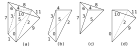
\includegraphics[width=\hsize]{triprism_decomp.eps}
\caption{三角柱を3つの四面体に分解}
\label{fig:triprism_decomp}
\end{center}
\end{figure}

前節まで扱ってきた1四面体要素のシミュレーションを本節では複数要素に拡張します。
任意の多面体を四面体に分解し,
それを組み合わせて連立一次方程式を構成します。
詳細を図\ref{fig:triprism_decomp}
に示す例とともに述べます。

図\ref{fig:triprism_decomp}(a)の三角柱が解くべき系の全体です。
これを一点鎖線で示す面で切断すると, (b), (c), (d), 3 つの四面体に分解できます。
これらの四面体がそれぞれ独立に前節までに示したような形状依存行列 $r$, $s$
を持ちます。
これらに添え字, ここでは$k$をつけて $r_k$, $s_k$
と書きます。$k=0, 1, 2$ をそれぞれ四面体 (b), (c), (d) に対応させます。
系全体で12本の辺があるため, ローカルな $r_k$, $s_k$ の要素を大きさが 12
であるグローバルな正方行列$R_k$, $S_k$に配置します。その配置を形式的に
\begin{align}
R_{k,g(k, l),g(k, m)} &= r_{k,l,m}\\
S_{k,g(k, l),g(k, m)} &= s_{k,l,m}
\end{align}
と書くことにします。$R$, $S$, $r$, $s$
について, 第一の添え字は要素番号, 第二の添え字は行番号,
第三の添え字は列番号を表すことにします。
$g$はローカルエッジ番号をグローバルエッジ番号に変換する関数です。
本章では番号の振り方は辞書順に統一するため,
本例では$g$は表\ref{tab:local2global}のようになります。
従って, 例えば$k=2$について
\begin{align}
R_2=
\left(
\begin{array}{ccccc|ccccc|cc}
r_{2,0,0} & 0 & r_{2,0,1} & 0 & r_{2,0,2} & 0 & 0 & 0 & r_{2,0,3} & 0 & r_{2,0,4} & r_{2,0,5}\\
0 & 0 & 0 & 0 & 0 &  0 & 0 & 0 & 0 & 0 &  0 & 0 \\
r_{2,1,0} & 0 & r_{2,1,1} & 0 & r_{2,1,2} & 0 & 0 & 0 & r_{2,1,3} & 0 & r_{2,1,4} & r_{2,1,5}\\
0 & 0 & 0 & 0 & 0 &  0 & 0 & 0 & 0 & 0 &  0 & 0 \\
r_{2,2,0} & 0 & r_{2,2,1} & 0 & r_{2,2,2} & 0 & 0 & 0 & r_{2,2,3} & 0 & r_{2,2,4} & r_{2,2,5}\\
\hline
0 & 0 & 0 & 0 & 0 &  0 & 0 & 0 & 0 & 0 &  0 & 0 \\
0 & 0 & 0 & 0 & 0 &  0 & 0 & 0 & 0 & 0 &  0 & 0 \\
0 & 0 & 0 & 0 & 0 &  0 & 0 & 0 & 0 & 0 &  0 & 0 \\
0 & 0 & 0 & 0 & 0 &  0 & 0 & 0 & 0 & 0 &  0 & 0 \\
r_{2,3,0} & 0 & r_{2,3,1} & 0 & r_{2,3,2} & 0 & 0 & 0 & r_{2,3,3} & 0 & r_{2,3,4} & r_{2,3,5}\\
\hline
r_{2,4,0} & 0 & r_{2,4,1} & 0 & r_{2,4,2} & 0 & 0 & 0 & r_{2,4,3} & 0 & r_{2,4,4} & r_{2,4,5}\\
r_{2,5,0} & 0 & r_{2,5,1} & 0 & r_{2,5,2} & 0 & 0 & 0 & r_{2,5,3} & 0 & r_{2,5,4} & r_{2,5,5}\\
\end{array}
\right)
\end{align}
となります。$k=0, 1$, そして$S_k$についても同様になります。

\begin{table}[tbp]
\caption{ローカルエッジ番号とグローバルエッジ番号の対応}
\label{tab:local2global}
\begin{center}
\begin{tabular}{|l|r|l|r|l|r|}
\hline
\multicolumn{2}{|c|}{$k=0$}&
\multicolumn{2}{|c|}{$k=1$}&
\multicolumn{2}{|c|}{$k=2$}\\
\hline
$g(0, 0)$ & 0 & $g(1, 0)$ & 3 & $g(2, 0)$ &  0 \\
$g(0, 1)$ & 1 & $g(1, 1)$ & 4 & $g(2, 1)$ &  2 \\
$g(0, 2)$ & 2 & $g(1, 2)$ & 5 & $g(2, 2)$ &  4 \\
$g(0, 3)$ & 3 & $g(1, 3)$ & 6 & $g(2, 3)$ &  9 \\
$g(0, 4)$ & 4 & $g(1, 4)$ & 7 & $g(2, 4)$ & 10 \\
$g(0, 5)$ & 5 & $g(1, 5)$ & 8 & $g(2, 5)$ & 11 \\
\hline
\end{tabular}
\end{center}
\end{table}

また, それぞれの四面体要素は独立に透磁率$\mu$, 誘電率$\epsilon$, 導電率$\sigma$
を持ちます。
これらに添え字, ここでは$k$をつけて
$r_k$, $s_k$%, $\mu_k$, $\epsilon_k$, $\sigma_k$
と書きます。このように定義した記号を使い,
\begin{align}
\left\{
\sum_k
\left[
{\mu_k}^{-1} R_k
-\omega\left(\omega\epsilon_k+j\sigma_k\right)S_k
\right]
\right\}
\bm{v}
=\sum_k \bm{e}_{1,k}+\sum_k\bm{e}_{2,k}+\sum_k\bm{e}_{3,k}
\end{align}
と構成した方程式を$\bm{v}$について解くことで解を求めることができます。
右辺は1要素シミュレーションと同様の電流励起です。

これを行うコードをリスト?に示します。
この関数を使用して図?に示す例題を1つずつシミュレーションしていきます。
